\documentclass[10.5pt, twocolumn]{article}

\usepackage[english]{babel}
\usepackage{graphicx}
\usepackage{imakeidx}
\usepackage{mathrsfs, amsmath}
\usepackage{systeme}
\usepackage{array}
\usepackage[utf8]{inputenc}
\usepackage{siunitx}
\usepackage{booktabs}
\usepackage{adjustbox}
\usepackage{geometry}
\geometry{a4paper,total={145mm,210mm}}
\usepackage{makecell}
\usepackage{afterpage}
\usepackage{listings}
\usepackage{subcaption}
\usepackage[toc,page]{appendix}
\usepackage[table]{xcolor}
\usepackage{pifont} % ding symbols
\usepackage{tikz}
\usepackage{changepage}
\usepackage{multirow} % multi row in tables
\usepackage{booktabs}
\usepackage{textcomp} % registered and copyright symbol
\usepackage{lscape} % vertical instead to horizontal
\usepackage{longtable} % for more page tables
\usepackage{eurosym}
\usepackage{lmodern}
\usepackage{amstext}
\usepackage{pdfpages} % import pdf pages
%\usepackage[hidelinks]{hyperref} % delete ugly hyperref borders of hyperlink
\usepackage{hyperref} % internal hyperlinks
\usepackage{titling} % titles
\usepackage{titlesec} % subtitles
\usepackage{blindtext} % for casual texts
\usepackage{dblfloatfix} % forces image at bottom in two-column files
\usepackage{gensymb} % standard unit of measurement
\usepackage{enumitem}

\DeclareRobustCommand{\officialeuro}{%
  \ifmmode\expandafter\text\fi
  {\fontencoding{U}\fontfamily{eurosym}\selectfont e}}



\makeindex[columns=2, title=Indice alfabetico, options= -s mystyle.ist, intoc]

\newcommand*{\Scale}[2][4]{\scalebox{#1}{\ensuremath{#2}}}
\renewcommand*\contentsname{Indice}
\newcommand*\NewPage{\newpage\null\thispagestyle{empty}\newpage}
\newcommand{\Virgolette}[1]{``#1''}
\newcommand*\circled[1]{\tikz[baseline=(char.base)]{
	\node[shape=circle,draw,inner sep=2pt] (char) {#1};}}
\newcommand{\tikzcircle}[2][red,fill=red]{\tikz[baseline=-0.5ex]\draw[#1,radius=#2] (0,0) circle ;}%command for draw text circle coloured
\def\changemargin#1#2{\list{}{\rightmargin#2\leftmargin#1}\item[]}
\let\endchangemargin=\endlist
\makeatletter
\let\originalpart=\part



\newcolumntype{C}[1]{>{\centering\arraybackslash}p{#1}}
\newcolumntype{L}[1]{>{\arraybackslash}p{#1}}
\newcolumntype{R}[1]{>{\raggedleft}p{#1}}
\newcolumntype{G}[1]{>{\centering\arraybackslash\columncolor{gray0}}p{#1}}

\definecolor{gray0}{gray}{0.9}
\definecolor{gray1}{gray}{0.7}
\definecolor{gray2}{gray}{0.4}

\lstset{
	literate = {α}{{$\alpha$}}1 {∆}{{$\Delta$}}1 {θ}{{$\theta$}}1 {η}{{$\eta$}}1 {→}{{$\rightarrow$}}1 {∂}{{$\partial$}}1, %tutti i simboli da usare come codice
	language = Mathematica % linguaggio
}
\hypersetup{
	citebordercolor=red
}


% ----- TITLE
\titleformat*{\section}{\Large\bfseries}
\title{
	\large{University of Trento}\\
	\normalsize{Master in Mechatronics Engineering}\\
	\vspace{0.2cm}
	\large{\textit{Modelling and Simulation of Mechatronics Systems}}\\
	\vspace{0.2cm}
	\Large{\textbf{Development, analysis and optimization of the performance of an innovative driving simulator}}\\
	\vspace{0.25cm}
	\hrule
	\vspace{0.2cm}
	\large{\textbf{Kinematics analysis}}\\	% Title
	\vspace{0.2cm}
	\hrule
}
\author{A. Comoretto \and J. Losi \and S. Valentini}
\date{\vspace{0.5cm}}
% ----- TITLE


\begin{document}
\maketitle

The kinematic analysis...

\section{Poisition analysis}
\label{s:Position}
In this section the mechanism's behaviour is studied.
In Figure \ref{f:Top-View} is shown the top view of the mechanism.
\begin{figure}[h!]
	\centering
	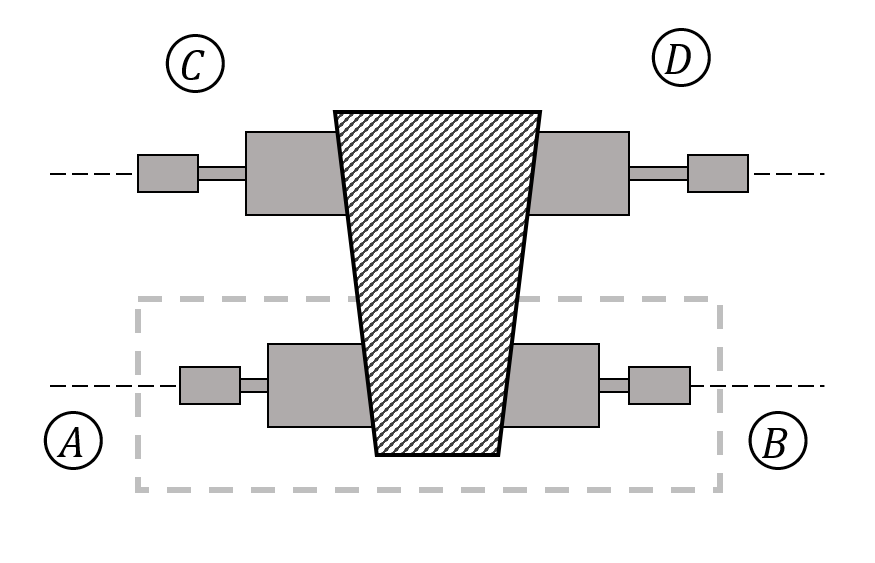
\includegraphics[width=7cm]{Images/Mechanism_TopView}
	\caption{Top view of the full-mechanism.}
	\label{f:Top-View}
\end{figure}

In first approximation a 2D analysis is conduced, and is refered only to the bodies \circled{A} and \circled{B}.

\subsection{Direct position analysis}
\label{s:Direct-position}
The mechanism studied in the 2D simplification is the marked part in Figure \ref{f:Top-View}, in fact only sub-mechanisms \circled{A} and \circled{B} are taken into account, and the result is shown in Figure \ref{f:2D_Mechanism}.
\begin{figure}[h!]
	\centering
	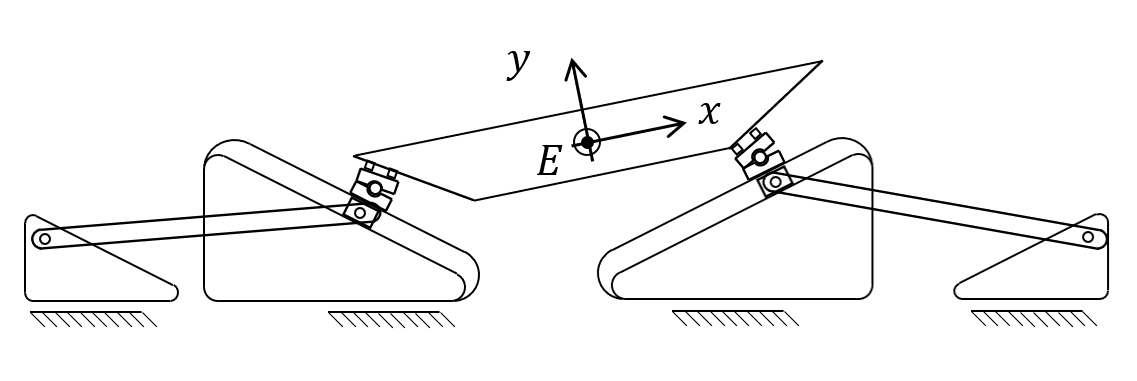
\includegraphics[width=7cm]{Images/Mechanism_LateralView}
	\caption{2D mechanism.}
	\label{f:2D_Mechanism}
\end{figure}

For the 2D analysis it is chosen to consider the length of the platform as a constant, even if it could be variable, due to its geometry.
More complex analysis are made in the following Section \ref{s:3D-kinematic} during the 3D analysis.

Thanks to this consideration it is possible to say that the full-mechanism is composed by two mirrored sub-mechanisms, made by four sub-bodies, joined by the platform.
So the sub-mechanism studied during the 2D kinematic analysis is shown in Figure \ref{f:Sub-Mechanism}.
\begin{figure*}[h!]
	\centering
	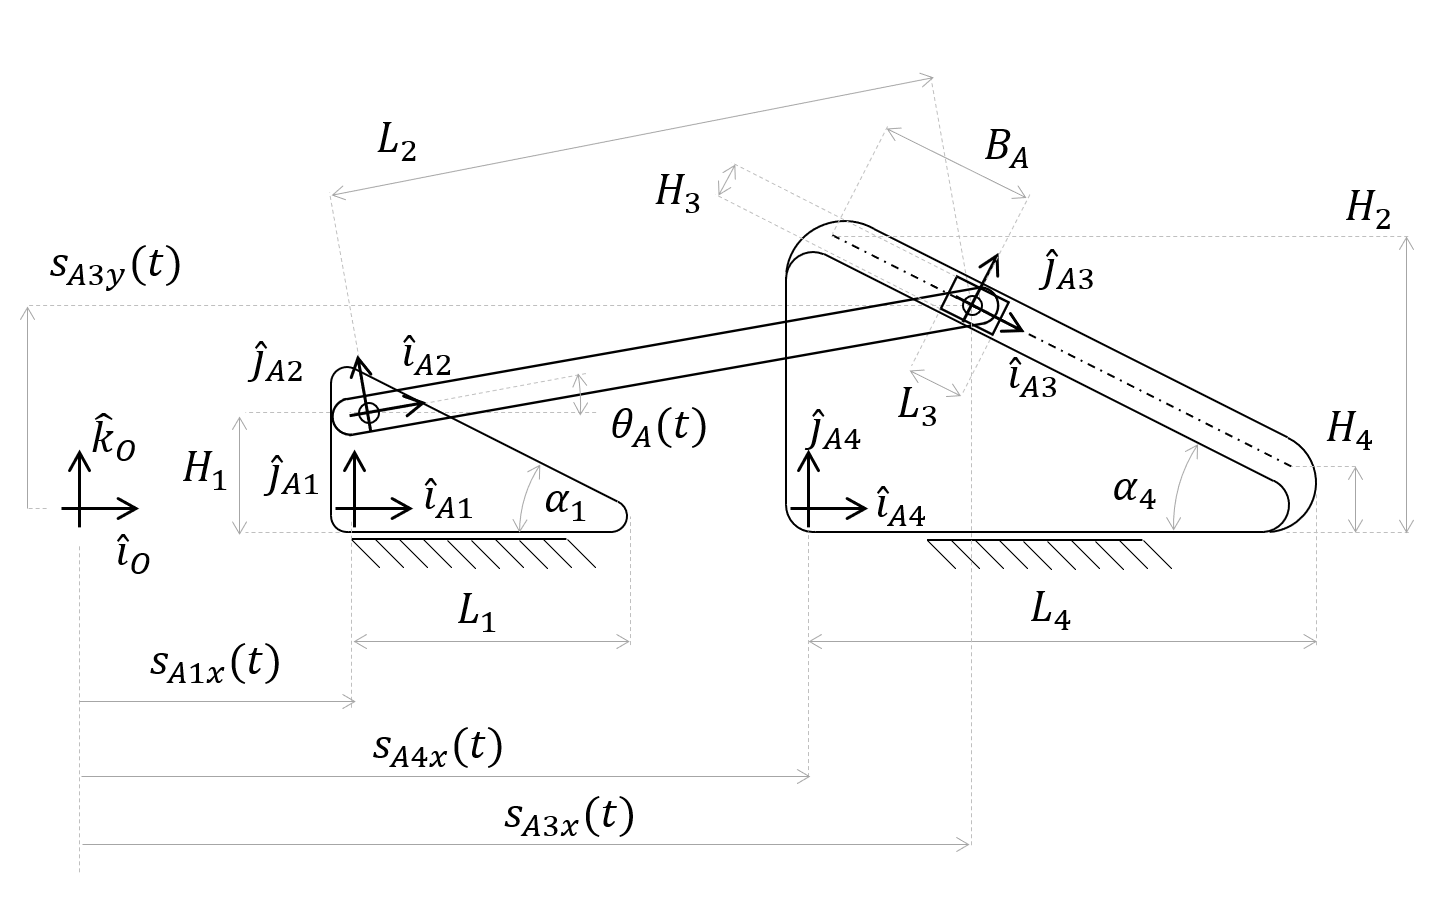
\includegraphics[width=12cm]{Images/Sub-Mechanism}
	\caption{One of the four sub-mechanism of the structure.}
	\label{f:Sub-Mechanism}
\end{figure*}
The same can be done for all the other sub-mechanisms by changing the subscripts.

At a first sight, it is easy to say that the four motors will be the independant variables, they are:
\begin{itemize}
  \item \( s_{A1x}(t) \);
  \item \( s_{A4x}(t) \);
  \item \( s_{B1x}(t) \);
  \item \( s_{B4x}(t) \).
\end{itemize}
Although the simplicity of this consideration it has to be revisited in way to work together with the previous one: in fact consider the length of the platform (named \( L_5\)) constant, means that one of the motor has to become a dependant variable.

In particular \( s_{B1x}(t) \) is considered the dependant variable, while the other three actuators consitute the independent variables set \( q_{I} \).

At the same time it has to be defined a set of dependant variables \( q_{D} \).
In particular for the description of the sub-mechanism's behaviour the following elements are chosen:
\begin{itemize}
  \item \( s_{A3x}(t) \) and \( s_{A3y}(t) \) which are the space coordinates of the body 3;
  \item \( \theta_A(t) \) which is the angle of the body 2;
  \item \( B_A(t) \) which is the distance of the body 3 from the upper-left edge of the body 4.
\end{itemize}

To write the kinematics equations, the chosen approach involves a combination of the recursive and global approaches. The actuators' variables are computed starting from two auxiliary reference frames (RF), one located to the left and one to the right of the fixed RF, as shown in \colorbox{yellow}{FIGURA}.\\
The mechanism is treated as the combination of two sub-systems \circled{A} and \circled{B}, each one them representing a closed loop from the kinematics point of view, solved using two recursive chains constrained at the inclined runner (body 3). Then, the last constraint equation is built up imposing that the platform links the two sub-systems.\\
This approach is particularly powerful, considering the simple symbolic expression that results from the inverse analysis carried on in Section \ref{s:Inverse-position}.

Solving the system of 6 constraints equations in 9 variables leads to a symbolic expression of the 6 dependent variables \( q_{D} \) as function of the actuators. The expression of the pose of the center of mass of the platform, treated as end effector (E) of the system, is derived from \( q_{D} \) by exploiting simple geometic considerations.

It's important to underline that the same procedure can be followed choosing \( s_{A1x}(t) \) instead of \( s_{B1x}(t) \) as powered off actuator, i.e. dependent variable. All the results showed in the next sections would be mirrored, due to the geometrical symmetry of the system.

The results of this Section are essential for the computation of the admittable extremes for the actuators, done in \ref{s:Extreme-positions}, and for the definition of the workspaces of the 2D-system, carried out in Section \ref{s:Position-workspaces}.

\subsection{Initial position problem}
\label{s:Initial-position}
The following is a simple criterion, based on geometrical considerations, for the determination of the initial values to be assigned to the actuators. The initial position is defined as follows:
\begin{equation}
  s_{A1x,0} = 0
\end{equation}
\begin{equation}
  s_{A4x,0} = \sqrt{L_2^2-\frac{H_2+H_4-2H_1}{4}} - \frac{L_4}{2}
\end{equation}
and the symmetrical happens for the fixed position for the sub-mechanism \circled{B} (\( s_{A1x,0} = s_{B1x,0} \) and \( s_{A4x,0} = s_{B4x,0} \)).

The complete formulation of the initial position involves also the definition of the distance \( L_e \) between left and right auxiliary RF and the fixed RF:
\begin{multline}
  L_e = 2*\sqrt{L_2^2-(\frac{H_2-H_4}{2}-H1+H4)^2}+\\
  + Q_3*\sin(\alpha_4)) + L_5
\end{multline}
that depends on the length of the platform \( L_5 \). Since the length of the platform, as it can be seen in Figure \ref{f:Top-View}, in general is variable from two values \cite{aVDS}, the initial position problem depends on it.

\subsection{Extreme positions problem}
\label{s:Extreme-positions}
A crucial part of the analysis deals with the definition of an automated way to determine the maximum range of variability of one actuator, say actuator 4 of \circled{B}, given any values of the other two. In general one could exploit the velocity analysis and determining the points at which the velocity ratios goes to infinity. Unfortunately this method is not effective, since inside these extremes there are configurations that implies compenetration of bodies.

Said so, a develpment of a consistent approach for the determination of the possible ranges of the actuators is considered necessary.\\
The developed criterion considers that:
\begin{itemize}
  \item the maximum and minimum position of the inclined runner through its seat is limited by limit switches positioned at an height of \( H_2 \) and \( H_4 \) respectively;
  \item the body 1 of each sub-system should not interpenetrate the body 4;
  \item the two bodies 4 of sub-systems \circled{A} and \circled{B}, i.e. the bodies below the platform, should not interpenetrate themselves.
\end{itemize}

The constraints are here summarized:
\begin{equation}
    s_{A1}x(t)+L_1 < s_{A4x}(t)+c_0
\end{equation}
\begin{equation}
    H_4 < s_{A3y}(t)
\end{equation}
\begin{equation}
   s_{A3y}(t) < H_2
\end{equation}
\begin{multline}
    s_{A4x}(t) < s_{A1x}(t)+\\
    +L_2 \cdot cos(arctan(\frac{H_2-H_1}{L_2}))
\end{multline}
\begin{equation}
   s_{A4x}(t)+s_{B4x}(t)+2 L_4 < L_e-c_1
\end{equation}
The same is applied for sub-mechanism \circled{B}.
Two variables, useful for the optimization part, are also introduced:
\begin{itemize}
  \item \( c_0 \): accepted interpenetration between bodies 1 and 4;
  \item \( c_1 \): minimum distance required between the two sub-mechanisms \circled{A} and \circled{B}.
\end{itemize}

For making this work in an automated way a Maple\textsuperscript{TM} function is written, \texttt{extremes(actuator, other\_actuators, data\_in, c0, c1)}, which returns a set containing the two lower and upper limits for \texttt{actuator} given \texttt{other\_actuators} representing the values of the other two.

\subsection{Position workspaces}
\label{s:Position-workspaces}
Following the approach introduced inthe first Paper \textit{"System requirements"}, in this Section the three workspaces regarding the 2D-system are obtained. In particular, considering the 3 DoFs, they are:
\begin{\begin{itemize}
  \item workspace between Sway (\( x \)) and Heave (\( y \));
  \item workspace between Sway (\( x \)) and Roll (around \( z \));
  \item workspace between Heave (\( y \)) and Roll (around \( z \));
\end{itemize}

The objective is to build the workspaces exploiting a solid method, that could be useful in more advanced analysis, such as the one of \ref{s:Parameters}.

At first,\( x-y\) workspace is defined by moving only one actuator at time, while others are mantained fixed at their initial position. The range of variability is defined by using \texttt{extremes} function described in \ref{s:Extreme-positions} and assigning the initial values. Nesting this approach in three \texttt{for} loops results in a cloud of points. Unfortunately, this approach is not effective, because for each \( (i j k) \)-th case in the loop, the ranges for the actuators are always the same (computed at the initial position).

\subsection{Inverse position analysis}
\label{s:Inverse-position}

\section{Velocity analysis}
Regarding the velocity analysis it was decided to operate in the following way.
At first, after have obtained from the position analysis the following three objects:
  \begin{itemize}
    \item \( \Phi_{tot}\): complete set of constraint equations;
    \item \( qI_{tot}\): set of independent variables;
    \item \( qD_{tot}\): set of dependent variables;
  \end{itemize}
three dependent variables (\( EE_{x}(t) \), \( EE_{y}(t) \) and \(EE_{angle}(t)\)) were added to the set of dependent variables and clearly to set of constraint equations. The aim was to obtain directly the velocity ratios related to these variables, that are the \( x \) position, the \( y \) position and the roll angle of the center of mass of the platform that was tought as the position of an eventual driving position.
If that had not been done , we would obtain velocity ratios related  to other internal variables, such as the angles of the bars and the positions of the rolleys.
At this point, in order to perform the Jacobians, we dropped the time dependency and after that, a function to restore the dependency w.r.t. the time was created, required to compute the derivation later.
Furthermore the Jacobians w.r.t. the dependent and independent coordinates has been computed and thus the matrix of velocity ratios \([ \tau ]\) was calculated exploiting the Jacobians.
Secondly it was developed the section for the plot of velocity ratios as a function of the independent variables, that are the position of the three actuators (because as already said, supposing a constant value of the length of the platform, one can be considered as \Virgolette{dummy}). In that section, not all the velocity ratios were plotted but only the ones related to the \( x \) and \( y \) position of the end effector and to its roll angle because those one were the only one really significative for our analysis.
Speaking about that section, a procedure for the plots called \texttt{velocity\textunderscore plot} was made. More specifically the procedure takes as inputs:
  \begin{itemize}
    \item \texttt{EE\textunderscore number}: chosen number between 1 and 3 that identifies the correct end effector variable (\( x \), \( y \) or angle);
    \item \texttt{actuator\textunderscore number}: desired actuator variable w.r.t whom it is chosen to plot the solution;
    \item \texttt{actuator\textunderscore extremes}: two elements vector that identifies the extreme postions of the desired actuator;
    \item \texttt{constant\textunderscore actuators\textunderscore values}: two values vector that identifies the values to be assigned by the two actuators that remain constant.
  \end{itemize}
It gives as outputs the trasmission ratios between \( x \), \( y \) position and angle of the end effector and the actuators as a function of one of the three independent DoF, assuming the other two as constants.
As third main point it was decided to plot, besides the velocity ratios, also the pure velocities of the \( x \), \( y \) position of the end effector and its roll angle w.r.t. the position of one of the three DoF. In that case, as the requests specified, the velocity of the active actuator was fixed to one while the position of the other two actuators was mantained in the initial position.
In order to develop this part, at first, it was calculated analitically the velocity of the dependent coordinates solving the derivative w.r.t. time of the equation of the complete set of constraints considering as unkonwns the derivative w.r.t. time of the complete set of dependent coordinates. Then, in the solution obtained, was substituted the chosen solution of the kinemtics found before.

\section{Acceleration analysis}
This part was quite similar to the one made before.
As a matter of fact, having the analitical solution of the kinematics, in order to obtain the expression of the acceleration of the dependent coordinates it was solved the double derivative w.r.t. time of the complete set of constraints considering as unkonwns the double derivative w.r.t. time of the complete set of dependent coordinates.
After that, the chosen solution of the kinematics was substituted into the expression of the dependent acceleration in order to obtain them as dependent only to the independent variables.
Moreover the acceleration of the \( x \), \( y \) coordinates and of the roll angle of the end effector was plotted w.r.t the position of each one of the three DoF (mantaining the other two fixed at each time). Furthermore, as the the requests specified, the velocity and the acceleration of the moving actuator, that was considered for each plot, were fixed to an unitaty value.
\section{Effects of the main geometrical parameters}
\label{s:Parameters}
By varying the position of the actuators it is possible to know which positions can be reached by the end effector, whose set is called \Virgolette{workspace}.
This is one of the main parameters analyzed during the design and modelling of the mechanism: in particular it is required to optimize the workspace and to make it widen to the maximum.

This procedure will lead to determine the geometrical values of the mechanism, which are, from Figure \ref{f:Sub-Mechanism}, \( L_1 \), \( H_1 \), \( L_2 \), \( H_2 \), \( L_4 \) and \( \alpha_4 \).








\begin{thebibliography}{}
\bibitem{aVDS}
\Virgolette{\textit{Advanced Vehicle Driving Simulator}}, \textsc{ABDynamics}.

\bibitem{CKAS}
\Virgolette{\textit{6DOF Motion System}}, \textsc{CKAS}.

\bibitem{Kasim}
M. Kasim A. J., \Virgolette{\textit{Design and development of 6-dof motion platform for vehicle driving simulator}}, Universiti Teknologi Malaysia.
\end{thebibliography}
\end{document}
